\documentclass[aspectratio=169]{beamer}
%
% Choose how your presentation looks.
%
% For more themes, color themes and font themes, see:
% http://deic.uab.es/~iblanes/beamer_gallery/index_by_theme.html
%
\mode<presentation>
%{https://writelatex.s3.amazonaws.com/vpzdvfpgmtcs/page/20577db5fb5206cebb645db53626924bd7e5686f.jpeg}
  \usetheme{Frankfurt}      % or try Darmstadt, Madrid, Warsaw, ...
  \usecolortheme{beaver} % or try albatross, beaver, crane, ...
  \usefonttheme{default}  % or try serif, structurebold, ...
  \setbeamertemplate{navigation symbols}{}
  \setbeamertemplate{caption}[numbered]{}
\setbeamertemplate{footline}[frame number]

\usepackage[english]{babel}
\usepackage[utf8x]{inputenc}
\usepackage{hyperref}
\usepackage{graphicx}

\title[GetL_Presentation]{Grammaires et Langages : Présentation}
\author{Equipe Minizza - H4111}
\institute{INSA de Lyon}
\date{Mardi 1 Mars}

\begin{document}

\begin{frame}
\titlepage
\end{frame}

% Plan proposé :
%
% 1. 


\section{Structures de données}
\subsection{Diagramme de classes}
\begin{frame}{Diagramme de classes}
\begin{center}
 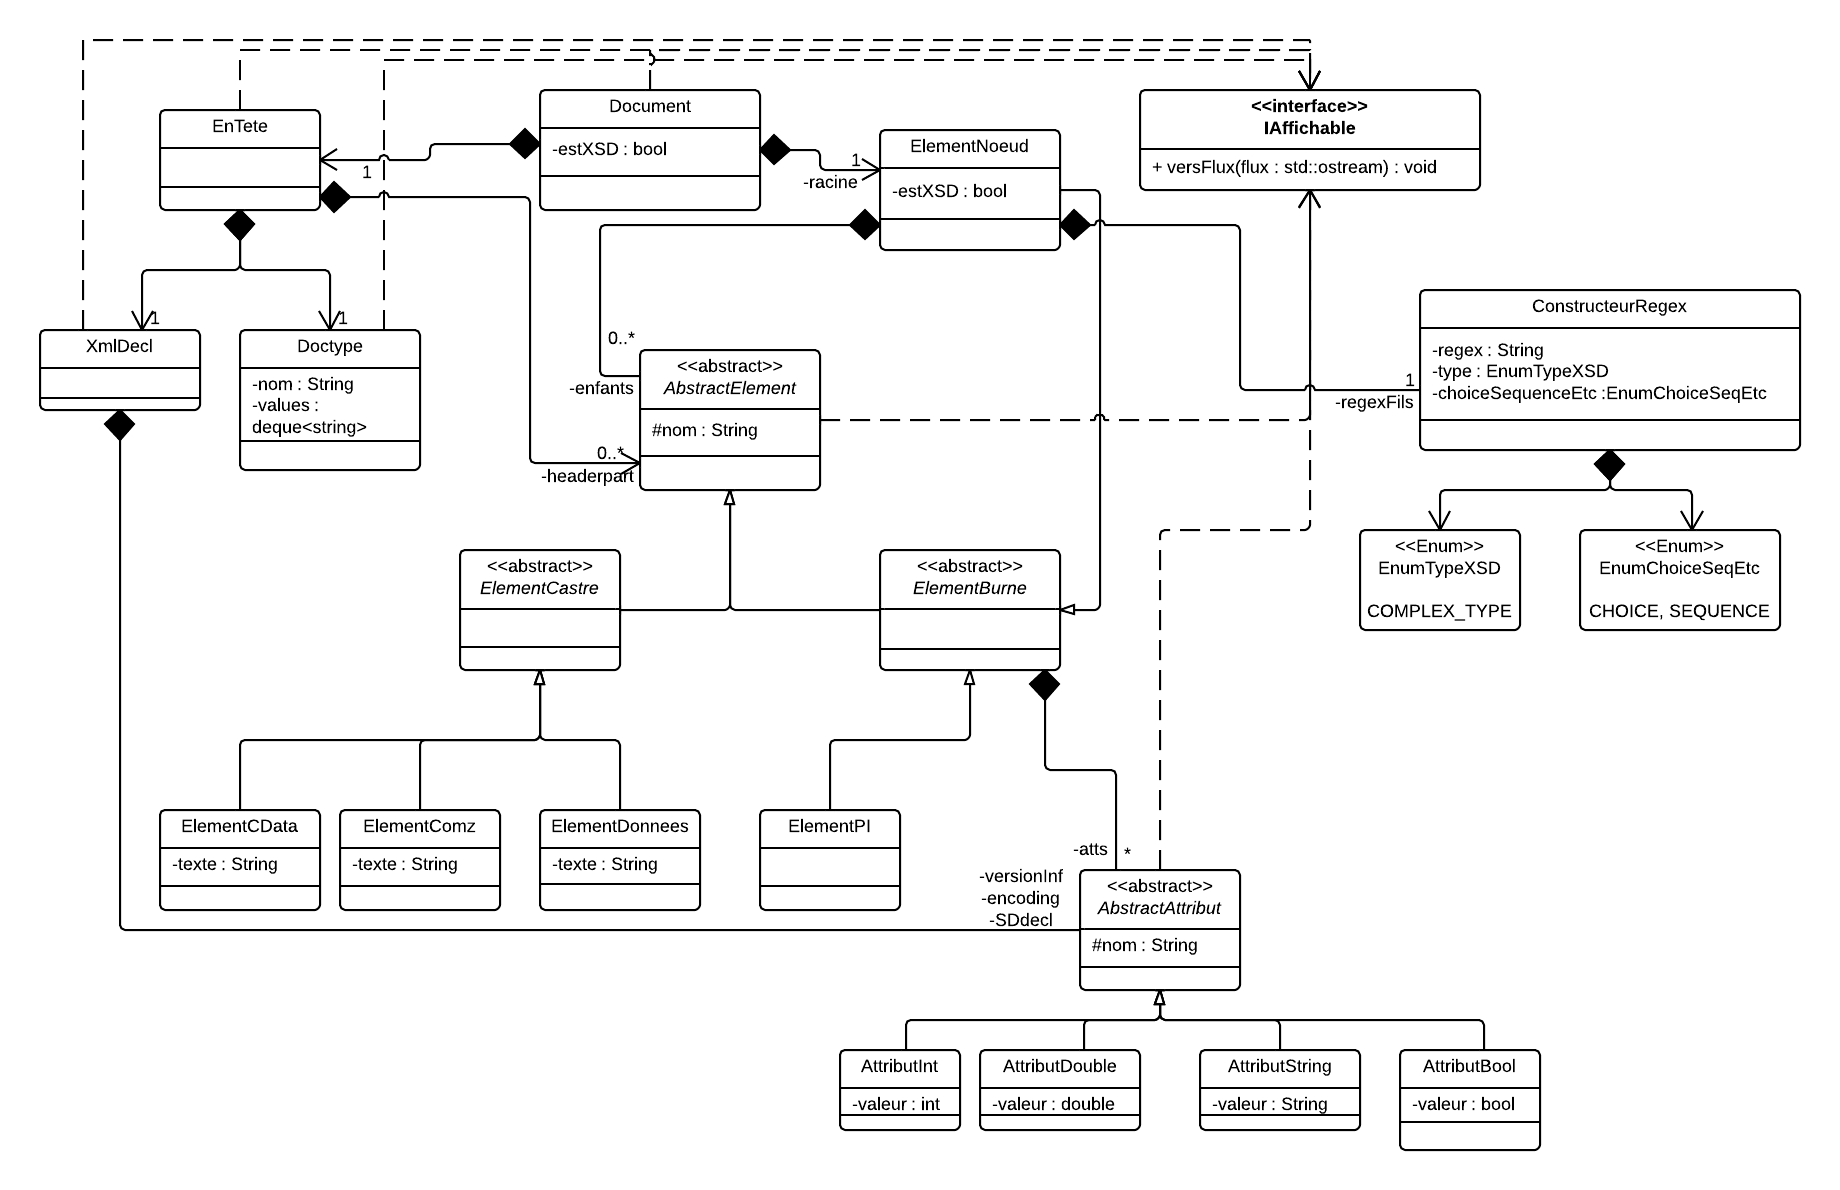
\includegraphics[scale=0.17]{diagdcla}
\end{center}
\end{frame}

\subsection{Diagramme de classes}
\begin{frame}{Diagramme de classes}
\begin{center}
  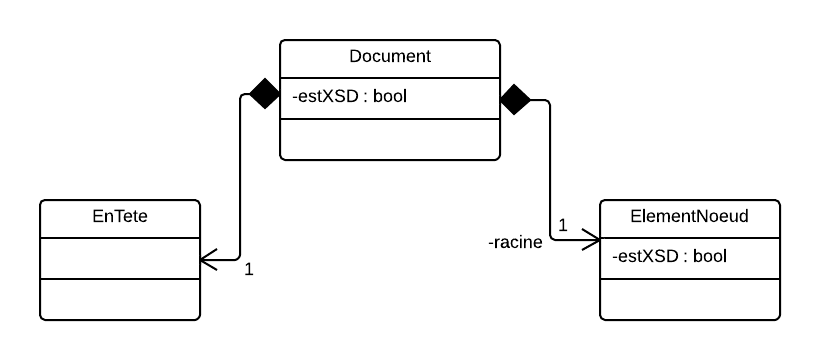
\includegraphics[scale=0.3]{ddc_doc}
\end{center}
\end{frame}

\subsection{Diagramme de classes}
\begin{frame}{Diagramme de classes}
\begin{center}
 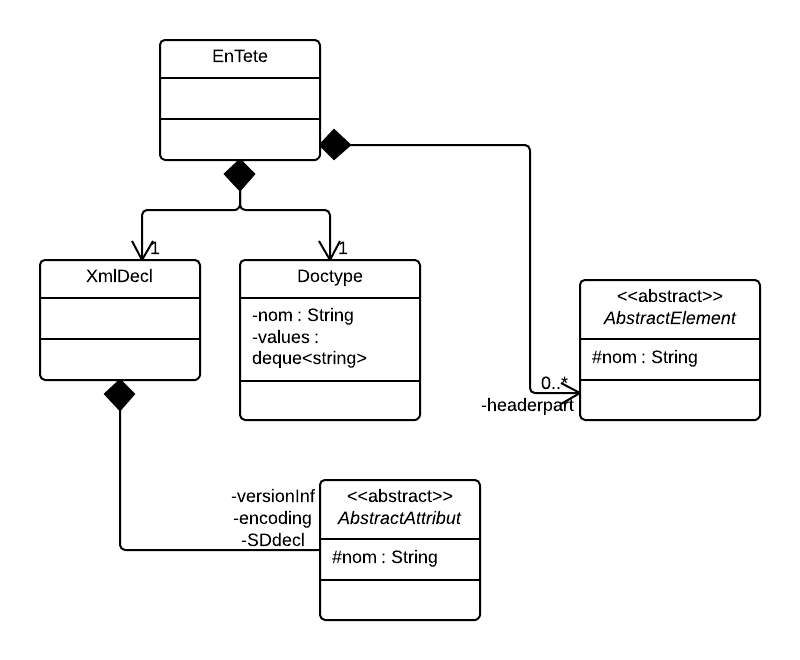
\includegraphics[scale=0.3]{ddc_ent}
\end{center}
\end{frame}

\subsection{Diagramme de classes}
\begin{frame}{Diagramme de classes}
\begin{center}
  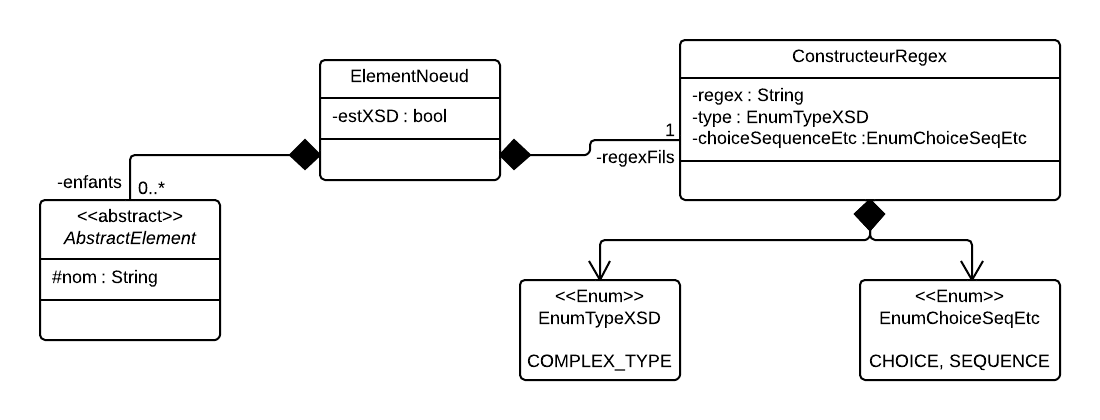
\includegraphics[scale=0.3]{ddc_noeud}
\end{center}
\end{frame}

\subsection{Diagramme de classes}
\begin{frame}{Diagramme de classes}
\begin{center}
  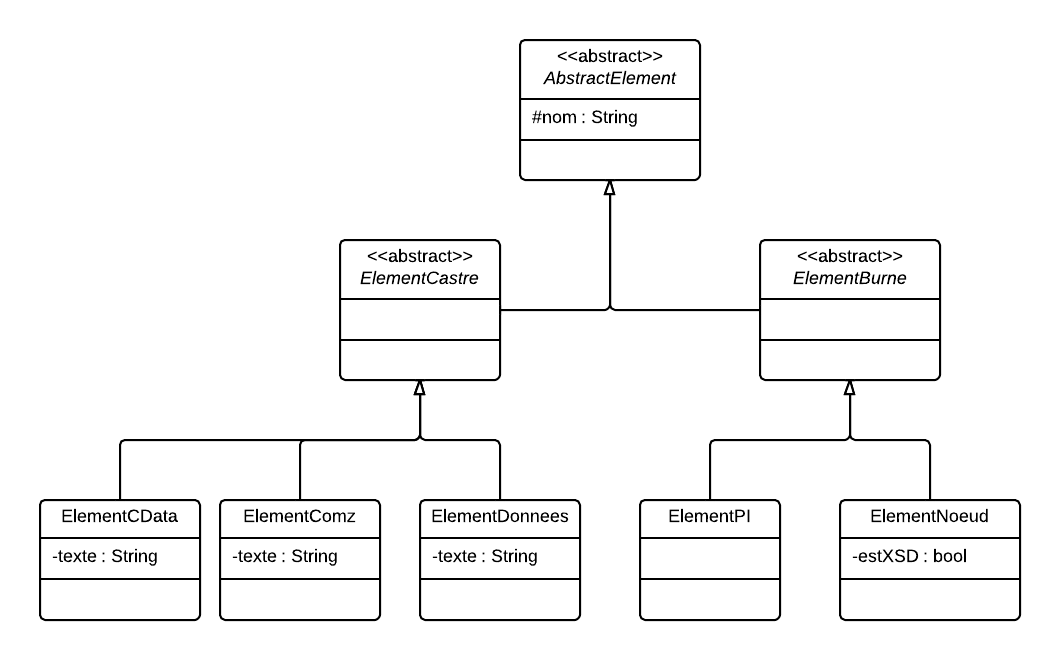
\includegraphics[scale=0.3]{ddc_abs_elmt}
\end{center}
\end{frame}

\subsection{Diagramme de classes}
\begin{frame}{Diagramme de classes}
\begin{center}
  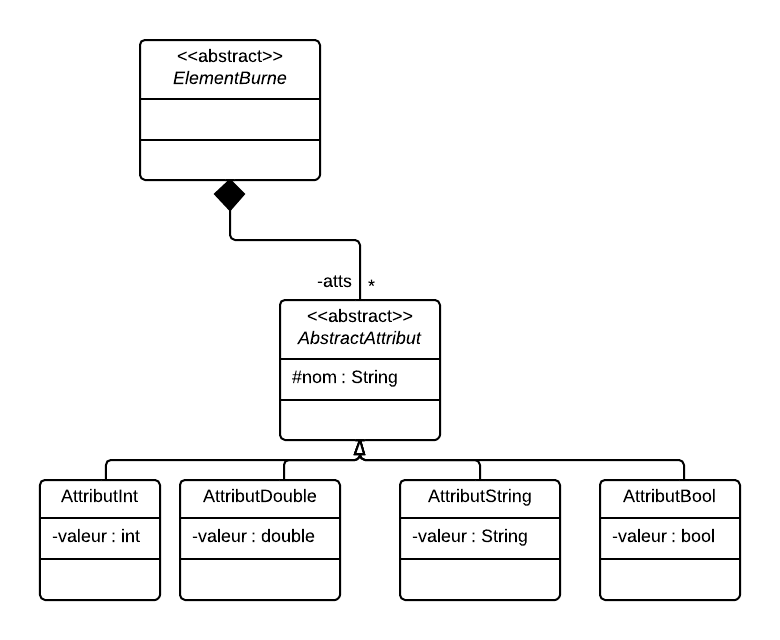
\includegraphics[scale=0.3]{ddc_elmt_burne}
\end{center}
\end{frame}

\subsection{Diagramme de classes}
\begin{frame}{Diagramme de classes}
\begin{center}
  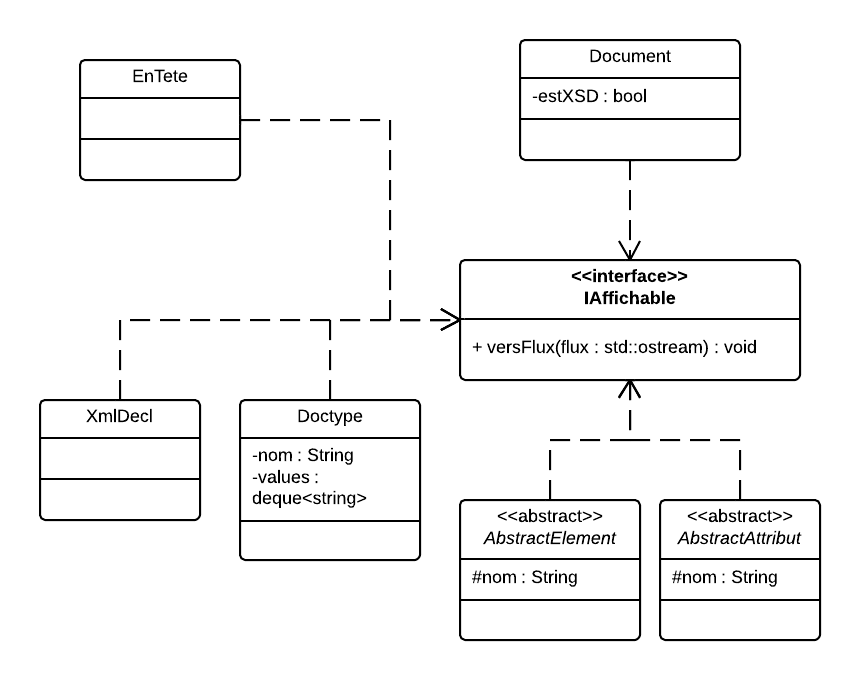
\includegraphics[scale=0.3]{ddc_iaff}
\end{center}
\end{frame}


\section{Algorithme de  validation}
\subsection{Algorithme de  validation}
\begin{frame}{Algorithme de validation}
 
\end{frame}

\section{Algorithme de transformation}
\subsection{Algorithme de  validation}
\begin{frame}{Algorithme de transformation}
 
\end{frame}


\section{Avancement du projet}
\subsection{Tout ce qui a été fait}
\begin{frame}{Tout ce qui a été fait}
 
\end{frame}

\subsection{Tout ce qui n'a pas été fait}
\begin{frame}{Tout ce qui n'a pas été fait}
 
\end{frame}

\section{Les tests}
\subsection{Ceux qui passent}
\begin{frame}{Ceux qui passent}
 
\end{frame}

\subsection{Ceux qui passent pas}
\begin{frame}{Ceux qui passent pas}
 
\end{frame}



\end{document}